\subsection{Approach}
The new vtkGPUVolumeRayCastMapper uses a ray casting technique ~\ref{raycasting} for volume rendering which is a state-of-the-art for volume rendering on modern graphics platforms. Algorithmically, at a high level, it is similar to the older version of this class (although with a fairly different OpenGL implementation since that original class was first written over a decade ago and used GPU assembly code).  One of the main reason we chose to use ray casting due to the flexibility of this technique, which enables us to support all the features of the software ray cast mapper but with the acceleration of the GPU. Ray casting is an image-order rendering technique, with one or more rays cast through the volume per image pixel. VTK is inherently an object-order rendering system, where the GPU renders all graphical primitives (points, lines, triangles, etc.) represented by vtkProp(s) in the scene in one or more passes (with multiple passes needed to support advanced features such as depth peeling for transparency).

The image-order rendering process for vtkVolume is initiated when the front-facing polygons of the volume’s bounding box are rendered with a custom fragment program. This fragment program is used to cast a ray through the volume at each pixel, with the fragment location indicating the starting location for that ray. The volume and all the various rendering parameters are transferred to the GPU through the use of textures (3D for the volume, 1D for the various transfer functions) and uniform variables. Steps are taken along the ray until the ray exits the volume, and the resulting computed color and opacity are blended into the current pixel value. Note that volumes are rendered after all opaque geometry in the scene to allow the ray casting process to terminate at the depth value stored in the depth buffer for that pixel (and, hence, correctly intermix with opaque geometry).

In addition to providing supported features of the old mapper, the new mapper added new capabilities such as clipping on GPU,  gradient opacity, and volume picking amongst many others. In the next few sections, we will cover each of these features in detail.

\subsubsection{Single Pass}
\begin{figure}
\centering
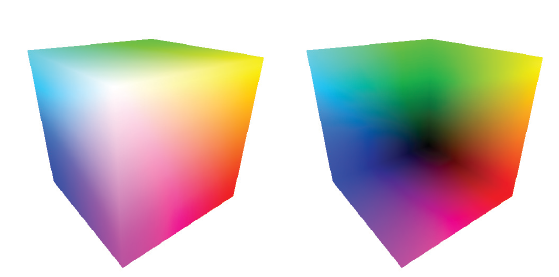
\includegraphics[width=3in]{frontandback.png}
\caption{Front and back faces are rendered for start and end position of the ray.}
\label{fig:raycasting}
\end{figure}


\begin{figure}
\centering
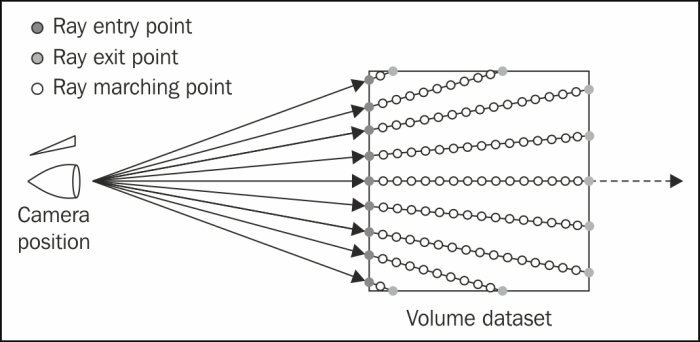
\includegraphics[width=3in]{raycasting.jpg}
\caption{Implementing volume rendering using single-pass GPU ray casting.}
\label{fig:raycasting}
\end{figure}

In a ray-casting algorithm, the entry and the exit point into the volume is needed to determine when to stop the ray-marching. To determine the entry and the exit point, one approach is to render the geometry of the volume bounding box of the volume twice. In the first pass, the front face of the geometry is rendered and in the second pass the backface is rendered as shown in ~\ref{fig:frontandback}. Using the interpolated vertex position and texture lookup, the start and end positions is computed. Instead of this, in vtkGPUVolumeRayCastMapper, entry and exit points are computed based on the fact that the texture extents of the volume is within vec3(1.0), vec3(-1.0) range (and ~\ref{fig:raycasting}). The code below is showing the fragment shader piece that determines whether or not to stop marching the rays depending on the value of stop.
 
 \begin{lstlisting}[breaklines=true]
 bool stop = any(greaterThan(g_dataPos, 
                 ip_texMax)) ||
             any(lessThan(g_dataPos, 
                 ip_texMin));
 \end{lstlisting}
 
 The advantage of such approach is that it requires one less pass and is faster than other approaches since there is no texture generation or lookup happens for determining the termination of the ray.
 
 
 \subsubsection{Dynamic Shader Generation}
 The first version of vtkOpenGLGPUVolumeRayCastMapper performed some operations on the CPU such as clipping while other operations on the GPU such as cropping of the volume. The new version replaced this behavior with all of the operations performed on the GPU. The advantage of this approach was a more streamlined code that is easier to maintain and debug. This approach also provided an opportunity to rework how to support different features without having too many branches in the shader code or having to send all the options to the shader because that would have been detrimental to the performance. In the new vtkOpenGLGPUVolumeRayCastMapper, the shader is dynamically composed by the mapper. For this to work, we have introduced tags in a vertex, or fragment shader which are then replaced by the vtkShaderComposer depending on the option enabled or chosen by the application code. For instance, the skeleton fragment shader defines tags as shown below:
 
//VTK::Base::Dec

//VTK::Termination::Dec 

At the run time then //VTK::Base::Dec is then replaced by the code shown below. 

To define a structure, we have chosen a strategy that separates the tags in found category: 

1. Declaration (:: Dec)
The tags belong to this group are meant to declare variables or function outside the main execution of the shader code. The variables defined are uniform, varying, and user-defined global variables. The functions defined are typically perform operations that are repetitive in nature such as computing color of a fragment. 

2. Initialization (:: Init)
The tags belong to this group are meant to initialize variables inside the main execution function of the shader but before the ray-casting loop in the fragment shader. An example of such code includes computation of the initial position of ray and direction of ray traversal.

3. Implementation (::Impl)
The tags belong to this group are the variables or functions or the combination of both that perform the actual operation of clipping, cropping, shading, etc. on one, two, or four component volume data. The implementation code used local and global variables and optimized for performance reasons as they are executed as long as the ray is traversing inside the volume and didn't run into a termination condition which is checked every time.  

4. Exit (:: Exit)
The tags belong to this group perform final computation such as the final color of the fragment. These tags are placed outside the ray-casting loop and typically contain numeric assignments.


 
 \subsubsection{Dual Depth Peeling}
 
 
 \subsubsection{Optimizations}